\section{Introduction}
This is the report of assignment1 for neural network design course.
The problem is to solve the two-spiral classification problem by implementing a multi-layer quadratic perception(MLQP) network with one hidden layer. I implement both online learning and batch learning ways to train the MLQPs model with the training data.
This report consists of derivation of the back-propagation algorithms for MLQPs, description of the implementation and the analysis of experiment result applying the model on the two-spiral problem.

%\begin{figure}
%\centering
%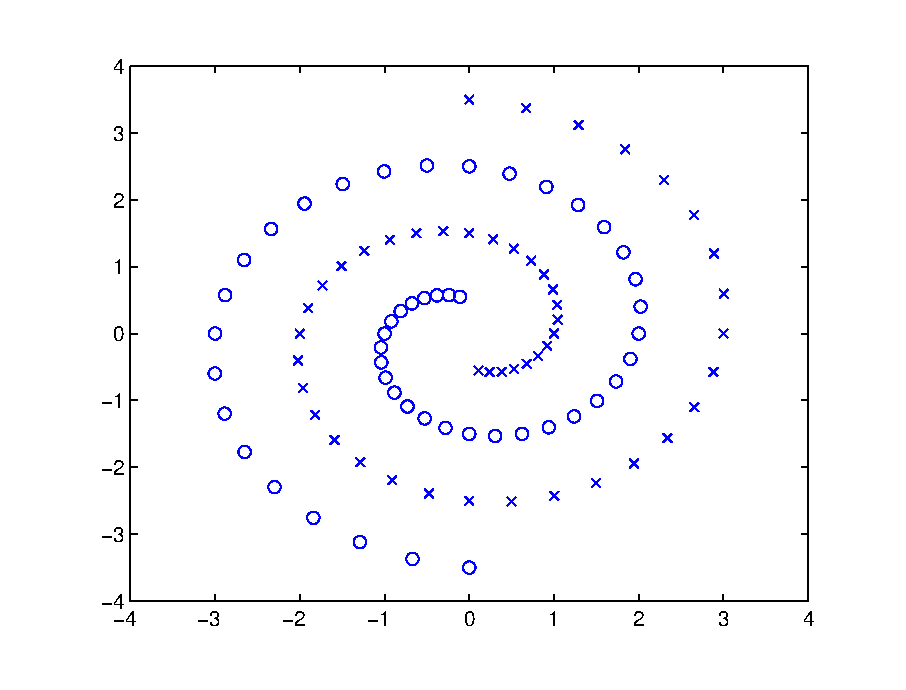
\epsfig{file=trainExamples.eps,width=0.9\columnwidth}
%\caption{Training set examples plotting}
%\end{figure}

